\documentclass[a4paper]{article}

\usepackage[pages=all, color=black, position={current page.south}, placement=bottom, scale=1, opacity=1, vshift=5mm]{background}
\usepackage[margin=1in]{geometry} % full-width

% AMS Packages
\usepackage{amsmath}
\usepackage{amsthm}
\usepackage{amssymb}
\backgroundsetup{contents={}}
\usepackage[spanish, es-tabla]{babel}


\renewcommand{\baselinestretch}{1.5}

% Unicode
\usepackage[utf8]{inputenc}
\usepackage{hyperref}
\hypersetup{
	unicode,
%	colorlinks,
%	breaklinks,
%	urlcolor=cyan, 
%	linkcolor=blue, 
	pdfauthor={Miriam Malament},
	pdftitle={Inversión en Capital Humano},
	pdfsubject={A simple article template},
	pdfkeywords={article, template, simple},
	pdfproducer={LaTeX},
	pdfcreator={pdflatex}
}

% Vietnamese
%\usepackage{vntex}

% Natbib
\usepackage[sort&compress,numbers,square]{natbib}
\bibliographystyle{mplainnat}

% Theorem, Lemma, etc
\theoremstyle{plain}
\newtheorem{theorem}{Theorem}
\newtheorem{corollary}[theorem]{Corollary}
\newtheorem{lemma}[theorem]{Lemma}
\newtheorem{claim}{Claim}[theorem]
\newtheorem{axiom}[theorem]{Axiom}
\newtheorem{conjecture}[theorem]{Conjecture}
\newtheorem{fact}[theorem]{Fact}
\newtheorem{hypothesis}[theorem]{Hypothesis}
\newtheorem{assumption}[theorem]{Assumption}
\newtheorem{proposition}[theorem]{Proposition}
\newtheorem{criterion}[theorem]{Criterion}
\theoremstyle{definition}
\newtheorem{definition}[theorem]{Definition}
\newtheorem{example}[theorem]{Example}
\newtheorem{remark}[theorem]{Remark}
\newtheorem{problem}[theorem]{Problem}
\newtheorem{principle}[theorem]{Principle}

\usepackage{graphicx, color}
\graphicspath{{fig/}}

%\usepackage[linesnumbered,ruled,vlined,commentsnumbered]{algorithm2e} % use algorithm2e for typesetting algorithms
\usepackage{algorithm, algpseudocode} % use algorithm and algorithmicx for typesetting algorithms
\usepackage{mathrsfs} % for \mathscr command

\usepackage{lipsum}

% Author info
\title{Retornos a la Educación e Inversión en Capital Humano:\\
El Caso Argentino}
\author{Miriam Malament\thanks{miriammalament@gmail.com}}
\date{\vspace{-5ex}}

\begin{document}
	\maketitle
	
	\begin{abstract}
     En este trabajo se presenta un análisis empírico de la situación laboral actual del país a los efectos de estimar los retornos a la educación en Argentina. Los datos provienen de la Encuesta Permanente de Hogares (INDEC) que corresponde al primer trimestre 2022. La metodología consiste en estimar las ecuaciones de Mincer total y computar los retornos, tanto bajo la hipótesis de retornos lineales por año de educación, como así también por máximo nivel alcanzado. Además, se examinará cómo ha variado la tendencia de los retornos a la educación en las últimas dos décadas y se intentará explicar alguna de las posibles causas.  
	\end{abstract}
	
	
% --------------------------
% Body matter
% --------------------------
\pagenumbering{arabic}			% arabic page numbering
\setcounter{page}{1}			% set page counter
	
	
\section{Introducción}
\label{sec:intro}

A partir de Gary Becker (1964), se ha desarrollado una rama de la literatura que entiende la decisión de educarse como un proyecto de inversión. Según su teoría, la educación traería aparejado múltiples beneficios como mayores salarios, menor tasa de desempleo, mejor salud y un efecto positivo sobre el capital humano de las futuras generaciones. Posteriormente, Jacob Mincer (1974) desarrolla una metodología econométrica para estimar los retornos a la educación que se ha aplicado en decenas de países con distintas culturas, recursos y sistemas económicos. Los resultados, según el país, pueden variar entre un 1,6\% de incremento en el salario por año adicional de educación en Afganistán, a un 22,4\% en Rwanda (Montenegro y Patrinos, 2014). 

La relevancia de Argentina como caso de estudio viene por el hecho de que su gasto en relación al PBI es uno de los más altos de la región y, siendo un país emergente, los salarios se ven perjudicados por las fluctuaciones económicas. Por lo tanto, este trabajo tiene por objetivo analizar los retornos a la educación siguiendo la ecuación de Mincer, para el 2022 en particular y la trayectoria temporal 2004-2022 en general, a partir de la microdata de la Encuesta Permanente de Hogares (EPH-INDEC). 

En la Sección 2 se introducirá el marco teórico, explicitando el modelo con el que se trabajará y se hará una breve revisión de la literatura acerca de qué es el capital humano, que implicancias tiene en el desarrollo económico y previas estimaciones de los retornos a la educación en Argentina y el mundo. En la Sección 3 se referirá a la situación del mercado laboral argentino y la distribución del ingreso desagregado por nivel educativo. En la sección 4 se abordarán los retornos a la educación, introduciendo el modelo y abordando ciertas cuestiones metodológicas del trabajo con los datos. Finalmente, la Sección 5 presentará los resultados y se concluirá en la Sección 6. 

\section{Marco Teórico}
\label{sec:marco_teorico}

La hipótesis del capital humano sugiere que la formación adquirida por las personas, ya sea en la educación formal o informal, es un capital y el proceso mediante el cual se acumula ese capital es la inversión en educación o conocimientos. Los principales exponentes de esta teoría fueron Gary Becker (1964), Jacob Mincer (1974) y Theodore Schulz (1961). En términos estrictamente económicos, inversión en capital humano destinando tiempo en educación formal e informal implica un sacrificio de consumo presente a los efectos de mejorar el perfil de ingresos esperados en el futuro (o ingreso permanente) que puede aumentar la capacidad de consumo futuro (Coremberg, 2010).

La evidencia empírica muestra una indiscutible relación positiva y significativa entre nivel educativo e ingresos laborales. Por lo tanto, la pregunta cuya respuesta divide la literatura en economía de la educación se refiere a la razón por la cual una persona que ha invertido más en educación percibe a lo largo de su vida un flujo de ingreso mayor que otra, idéntica en todo, pero que ha invertido menos. Los pioneros en este campo de estudio sostienen que la educación acrecienta la productividad del trabajador lo que, bajo ciertos supuestos acerca de la estructura del mercado de trabajo, termina impactando positivamente sobre los ingresos que percibe. En suma, los individuos ganan más porque son más productivos y lo que los hace más productivos son estas habilidades y conocimientos llamados “capital humano” (Paz, 2009).

Esta teoría del capital humano asume que la cantidad de educación, \textit{s}, se elige de manera de maximizar el valor esperado de los flujos futuros de ingreso w, hasta que uno se jubila, \textit{T}, neto de los costos de educación $c_s$. Por tanto, el s óptimo es aquel para el cual el ingreso marginal de un año adicional de educación es igual al costo marginal de dicho año (Adrogue, 2006). En el óptimo: 

\begin{equation*}
    \sum^{T-s}_{t=1} \frac{w_s-w_{s-1}}{(1+r_s)^t}
\end{equation*}

Siendo r la tasa de retorno. Si T es suficientemente grande, el lado izquierdo de la relación de equilibrio se puede aproximar de manera que la condición de equilibrio se traduce en
\begin{equation*}
 \frac{w_s-w_{s-1}}{r_s}=w_{s-1}+c_s
\end{equation*}

Si $c_s$ es suficientemente pequeño, se puede reordenar la expresión y obtener:

\begin{equation*}
 r_s \approx \frac{w_s-w_{s-1}}{w_{s-1}}\approx \log w_{s}+\log w_{s-1}
\end{equation*}

Se podrían estimar los retornos a s analizando como el logaritmo de los ingresos varía con s. Uno de los primeros trabajos que evaluó empíricamente dichos retornos fue el de Jacob Mincer (1974), que postuló una ecuación que relacionaba los ingresos ($W_i$) con
los años de educación ($s_i$), la experiencia ($X_i$), la experiencia al cuadrado ($X_i^2$ ) y las otras
variables observables que afectan los ingresos, diferentes de la experiencia1 y la educación ($X_i$). El término referido a la experiencia al cuadrado se incorporó para capturar la concavidad del perfil de ingresos, es decir, que con el correr de los años, los ingresos aumentan pero en menor proporción.

\begin{equation*}
    LnW_i=\alpha+\beta_1S_i+\beta_2X_i+ \beta_3X^2_i+\mu_i
\end{equation*}

en donde el término $\mu_i$ es un término de perturbación aleatoria y representa todas aquellas variables no observables que no están explícitamente incorporadas en la ecuación y que afectan los ingresos de los individuos. 

Las críticas a esta postura provienen de fuentes diversas. Un conjunto de trabajos surgido principalmente durante la primera mitad de la década de 1970, han apuntado su crítica a la hipótesis de capital humano aduciendo que si bien la educación y los ingresos monetarios están altamente relacionados, podría tratarse de una relación espuria. Podría ocurrir, por ejemplo, que los individuos innatamente más hábiles estudien más y permanezcan más tiempo (deserten menos) en el sistema educativo justamente por ser más hábiles que el resto. A la vez podría suceder que esa capacidad innata sea la que los conduzca a ser más productivos en sus empleos y que ello termine impactando positivamente en sus ingresos monetarios. Es decir, sería la habilidad innata la que haría estudiar más a los individuos y también sería la fuente de la mayor productividad e ingresos monetarios (Griliches, 1977; Card, 1994).

Pero si esto fuera efectivamente así todavía restaría contestar por qué los individuos más hábiles incurren en el costo que implica la acumulación de capital humano si lo que premia el mercado es su habilidad y no la educación adquirida. Arrow (1973) y Spence (1973), entre tantos otros, advirtieron que la inversión en educación es una de las maneras menos costosa para individuos y firmas de resolver un problema de asimetría de información en el mercado laboral. Los empleadores desconocen la productividad de los trabajadores que contratan y apelan a indicadores y señales para detectar esa productividad. Los trabajadores más productivos, por su parte, encuentran en la educación una señal importante para diferenciarse de los trabajadores menos productivos. A su vez, el costo de producir esa señal está inversamente relacionado con la capacidad de los agentes, por lo que a los más productivos puede quizá reportarles ganancias invertir en generarla.

Por otra parte, en términos macroeconómicos, la educación cumple un rol fundamental en la habilidad de un país emergente para absorber tecnología moderna y desarrollar la capacidad de crecimiento y desarrollo sostenible. De hecho, tanto la educación como la salud son mucho mayores en los países de mayores ingresos y se puede pensar que la causalidad es en ambas direcciones: con mayores ingresos, tanto las personas como el gobierno pueden pagar más en educación y salud y, con mejor educación y salud, mayor productividad e ingresos. Por lo tanto, como política pública, la estrategia debe enfocarse en ingreso, salud y educación de manera simultánea (Todaro y Smith, 2020).

De la misma manera que con capital físico, después de la inversión inicial, un flujo de ingresos futuros más altos se da a partir de la mejora en educación y salud. Por lo tanto, la tasa de retorno puede ser deducida y comparada con la de otras inversiones. Esta se estima a partir del valor presente descontado del incremento en el ingreso posible por la inversión y compararlo con los costos directos e indirectos. 

\begin{figure}[h]
    \centering
    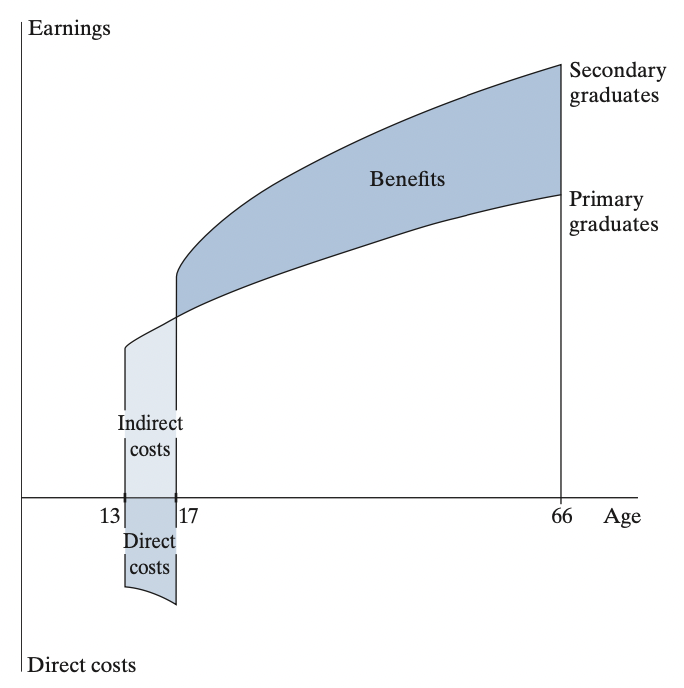
\includegraphics[scale=0.7]{figuras/Costos y beneficios de invertir.png}
    \caption{Costos y Beneficios Directos e Indirectos de Educación}
    \label{fig:my_label}
\end{figure}

Típicamente, en países emergentes, los costos sociales de educarse (el costo de oportunidad de la sociedad en su conjunto resultando de la necesidad de financiar la expansión educativa de niveles superiores cuando podrían ser usado de manera más productiva en otros sectores de le economía) aumentaría rápidamente mientras los estudiantes van llegando a niveles educativos más altos. Los costos privados de educación, en cambio, son aquellos pagados por los estudiantes por sí mismos, y aumentan de manera menos pronunciada (o incluso podrían decaer). Esta brecha entre costos sociales y privados provee más estímulos para demandar educación avanzada con respecto a demandar educación básica. El problema es que las oportunidades pueden ser acomodados para estas demandas distorsionadas solo en el costo social completo. 

\begin{figure}[h]
    \centering
    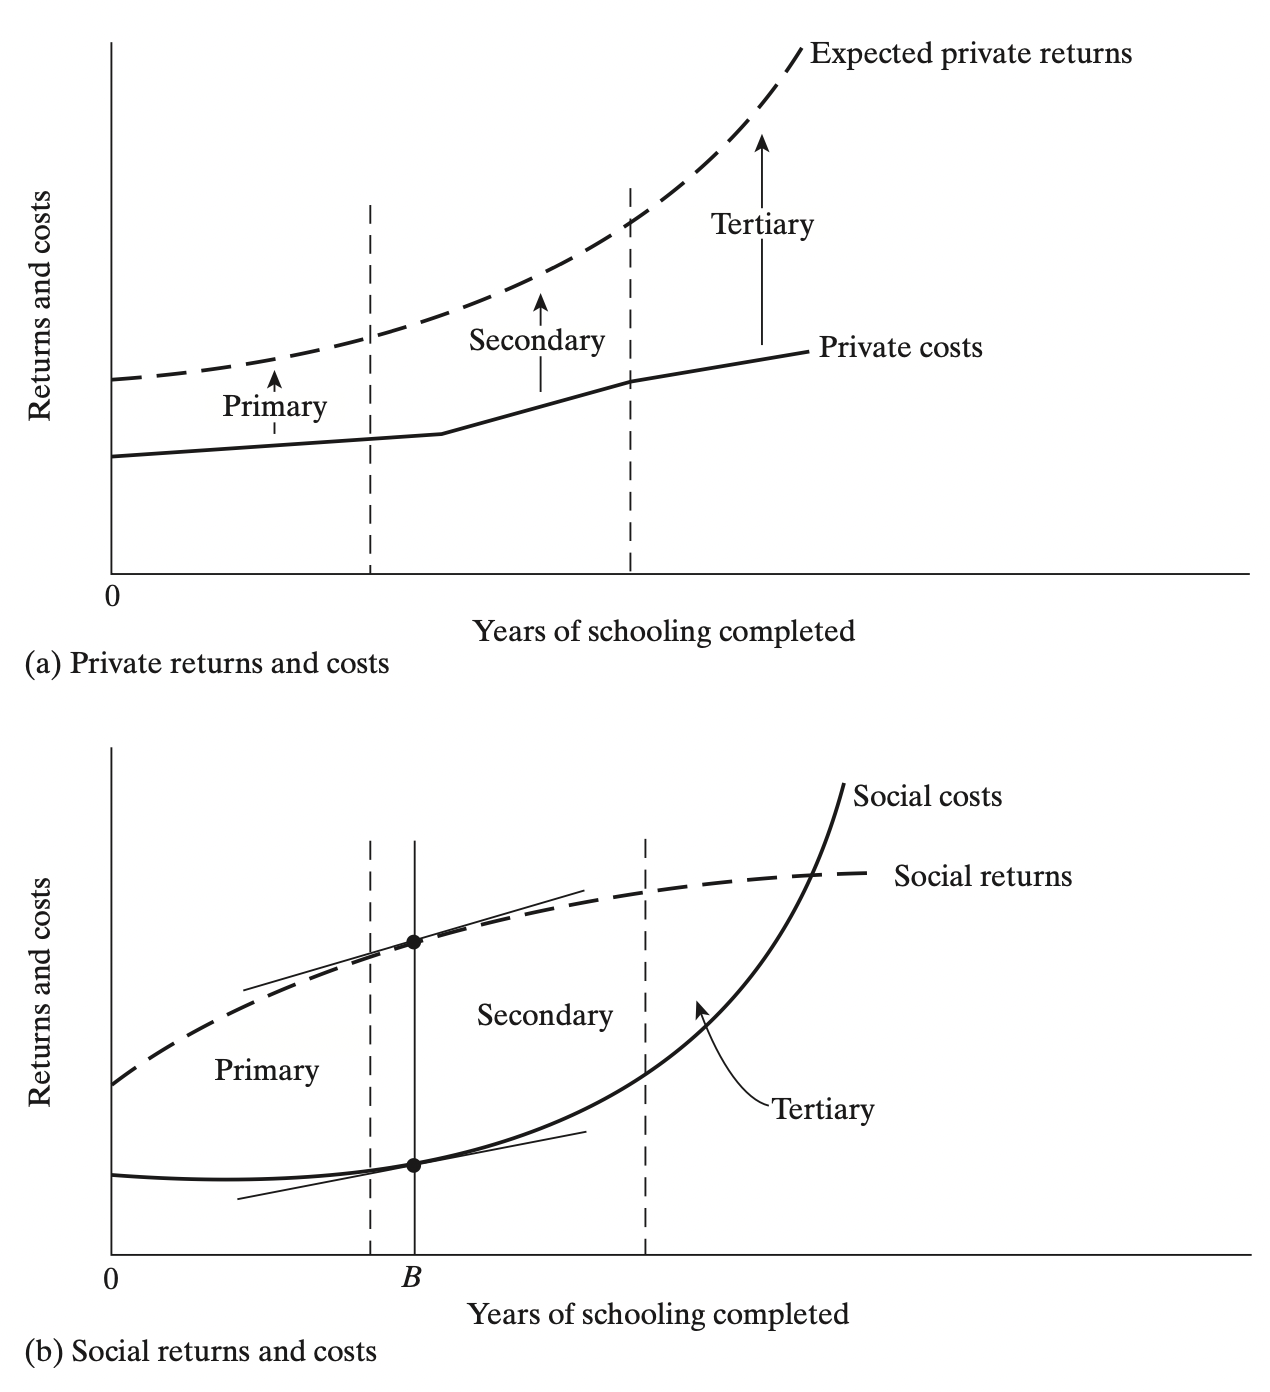
\includegraphics[scale=0.3]{figuras/costo-beneficio educarse.png}
    \caption{Retornos y Costos de Educación}
    \label{fig:my_label}
\end{figure}


Como señala la Figura 2, el beneficio social aumenta fuertemente al principio, reflejando niveles de productividad más altos a partir de la alfabetización y habilidades aritméticas básicas. Luego, el beneficio social marginal de cada año adicional de educación aumenta más lentamente y la curva de retorno social se va estabilizando. Por contraste, el costo social aumenta lentamente para niveles elementales de educación y mucho más rápidamente para niveles más avanzados. Este aumento rápido en el costo marginal social de educación post primaria es el resultado de un capital mucho más caro y de costos corriente de educación avanzada (infraestructura y equipamiento) y el hecho de que la educación post primaria en países emergentes está altamente subsidiado. 

En la siguiente tabla podemos observar los retornos a la educación de las distintas regiones: 

\begin{table}[h]
    \centering
    \includegraphics[scale=0.4]{figuras/retornos a la educación por region.png}
    \caption{Retornos a la Educación por Región}
    \label{fig:retornos_por_region}
\end{table}

Como se puede observar en esta tabla, existe evidencia empírica acerca de la existencia de diferencias en los retornos a la educación para hombres y mujeres. Por un lado, las mujeres tienen retornos a la educación más altos que los hombres en la mayoría de países desarrollados. Esto puede explicarse, en parte, debido a que con menos mujeres inscriptas, la mujer marginal que se inscribe tiende a ser más talentosa que el varón marginal. Aumentar la educación de mujeres no solamente aumenta su productividad y salarios, sino también aumenta la participación laboral femenina, el matrimonio, disminuye la fertilidad y aumenta fuertemente la salud y nutrición de los hijos, beneficiando así a las futuras generaciones también (Borjas, 2020).  

\section{El Mercado Laboral Argentino}
\label{sec:metodologia}

Esta sección tiene por objeto demostrar empíricamente que a mayor nivel educativo, mayores ingresos y menor desigualdad. Para ello, se realizó un análisis cuantitativo\footnote{Código del análisis cuantitativo en \hyperref[https://github.com/miriammalament22/development]{https://github.com/miriammalament22/development}} de los datos de la Encuesta Permanente de Hogares (EPH-INDEC) del primer trimestre del 2022\footnote{La EPH se actualiza cada seis meses y la del primer trimestre del 2022 era la última disponible al momento de comenzar el análisis cuantitativo en octubre 2022.}

\subsection{La Encuesta Permanente de Hogares}
\label{sec:metodologia:sec1}

La Encuesta Permanente de Hogares (EPH) es un programa nacional de producción sistemática y permanente de indicadores sociales llevado a cabo por el Instituto Nacional de Estadística y Censos (INDEC), que permite conocer las características sociodemográficas y socioeconómicas de la población. Es realizada en forma conjunta con las Direcciones Provinciales de Estadística (DPE).Tiene por objetivo central caracterizar la situación social de los individuos y las familias teniendo en cuenta las modalidades de su inserción en la estructura económico-social. Proporciona las tasas oficiales de actividad, empleo, desocupación y subocupación, los indicadores de pobreza e indigencia y otros resultados sobre las características socioeconómicas de la población.

En cuanto a su cobertura geográfica, abarca 31 aglomerados urbanos donde habita, aproximadamente, el 70\% de la población urbana del país. Cubre todas las capitales de provincia y aglomerados urbanos de más de 100 mil habitantes. Su periodicidad es trimestral. Por lo tanto, se realizan 4 estimaciones por año de los principales indicadores del mercado de trabajo.

Por otra parte, la EPH es una encuesta por muestreo. Esto significa que para conocer las diversas características del total de los hogares, se encuesta una pequeña fracción representativa de los mismos. Todas las muestras presentan limitaciones, errores de muestreo, que se producen porque las observaciones se realizan únicamente en una muestra y no en toda la población.

Los hogares que serán encuestados son seleccionados de forma aleatoria en dos etapas de selección: 
\begin{enumerate}
    \item Dentro de cada aglomerado, se selecciona una cantidad de radios censales o subdivisiones de los mismos (áreas).
    \item Se listan todas las viviendas particulares de las aéreas seleccionadas, para efectuar a partir de ese listado una selección aleatoria de viviendas. Los hogares que habitan esas viviendas son los hogares a encuestar.
\end{enumerate}   

Por lo tanto, existe un esquema de rotación 2-2-2 (la vivienda entra dos trimestres consecutivos - descansa dos trimestres consecutivos - vuelve a la muestra dos trimestres consecutivos)

Se va a estar trabajando con \textit{CH04} (género), \textit{CH06} (edad), \textit{NIVEL\_ED/CH12} (máximo nivel educativo alcanzado), \textit{ESTADO} (condición de actividad), \textit{P21} (monto de ingreso de la ocupación principal) y sus respectivos ponderadores \textit{PONDERA} y \textit{PONDIIO}. 

\begin{figure}[h]
    \centering
    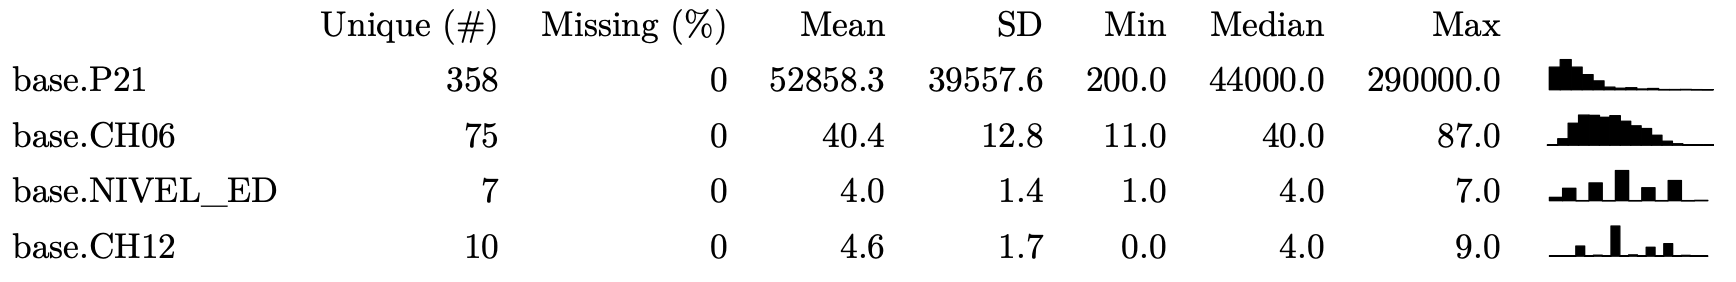
\includegraphics[scale=0.5]{figuras/estadisticas_descriptivas.png}
    \caption{Estadísticas descriptivas de las variables a utilizar}
    \label{fig:kernel_ingreso_genero_nivel_ed}
\end{figure}




\subsection{Distribución del Ingreso y Educación}
\label{sec:metodologia:sec4}

Podemos analizar empíricamente la distribución del ingreso utilizando los datos de ingreso que provee la EPH. De todas formas, se deben tomar dos precauciones. Por un lado, el 75\% los empleados declara cuáles son sus ingresos laborales y, por el otro, tiende a haber una subdeclaración especialmente en el estrato superior de los ingresos. 

En la Figura \ref{fig:distribucion_del_ingreso}, se puede observar la distribución del ingreso laboral (P21) en Argentina ponderada por PONDIIO (ponderador para los ingresos laborales). La distribución tiene su moda inclinada hacia la izquierda. 

Resulta relevante destacar que el ingreso medio se encuentra alrededor de los \$50.000. Si se toma en cuenta el dólar paralelo a inicios del 2022 (1 usd = \$180 arg), entonces el ingreso laboral promedio se encontraba por debajo de los \$300 dólares. 

\begin{figure}[h]
    \centering
    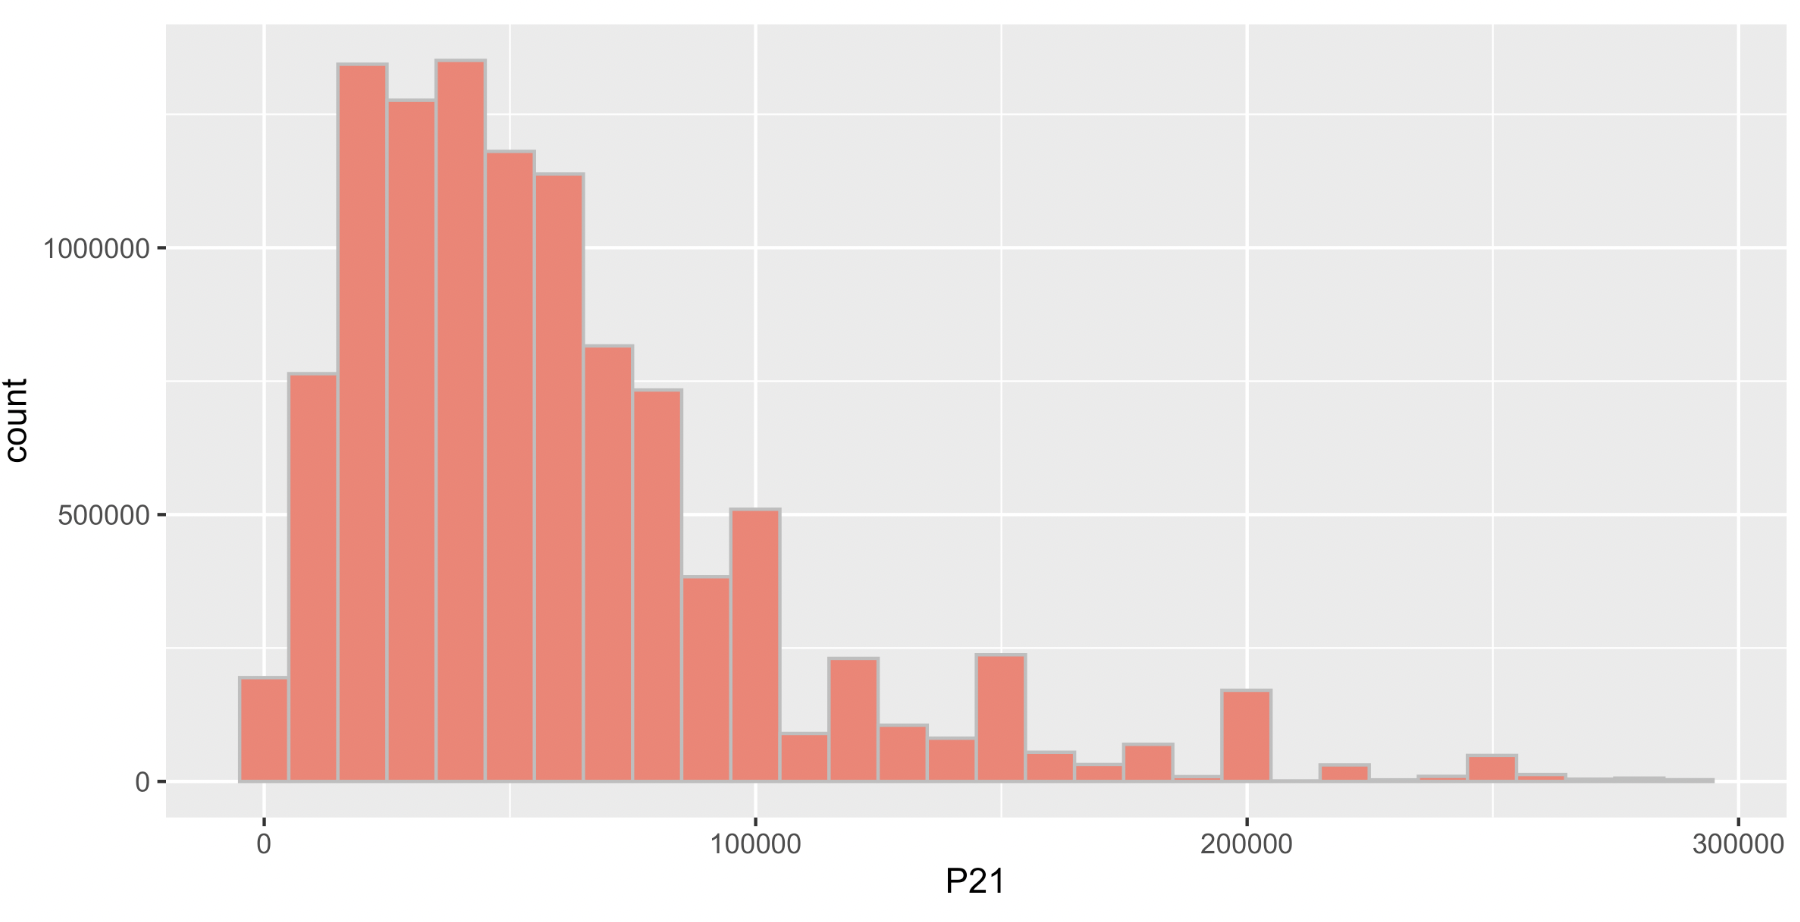
\includegraphics[scale=0.4]{figuras/Histograma.png}
    \caption{Distribución del ingreso}
    \label{fig:distribucion_del_ingreso}
\end{figure}

A los efectos de este trabajo, es necesario desagregar la distribución del ingreso de manera tal de demostrar que a mayor nivel educativo alcanzado, en promedio, mayores salarios. Por lo tanto, podemos desagregar el histograma de Figura 6 por nivel educativo como muestra la siguiente figura: 

\begin{figure}[h]
    \centering
    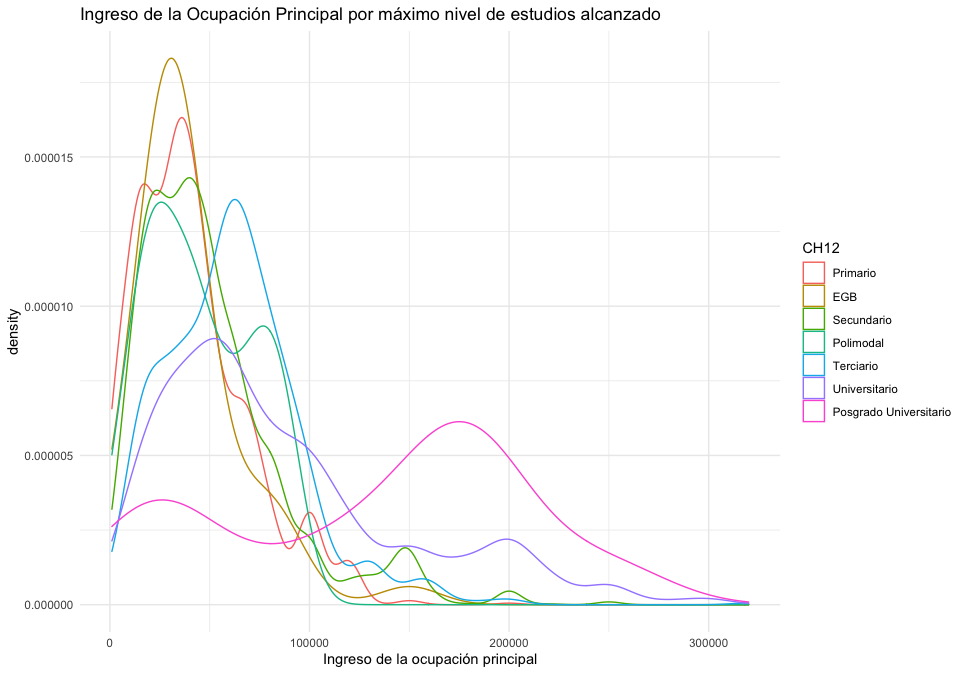
\includegraphics[scale=0.28]{figuras/distribucion_densidad_ingreso_ch12.png}
    \caption{Distribución del ingreso por nivel educativo}
    \label{fig:distribucion_del_ingreso_por_ch12}
\end{figure}

A partir de la Figura \ref{fig:distribucion_del_ingreso_por_ch12}, se puede concluir que a mayor nivel educativo, más se asemeja a una normal la distribución del ingreso. Esto quiere decir que a mayor nivel educativo, menos desigualdad. 

Esta conclusión se refuerza al desagregar por género como muestra la Figura     \ref{fig:kernel_ingreso_genero_nivel_ed}. 
Lo interesante es que, si existiese una brecha salarial entre hombres y mujeres, a mayor nivel educativo, menor es esta brecha. 
\begin{figure}[h]
    \centering
    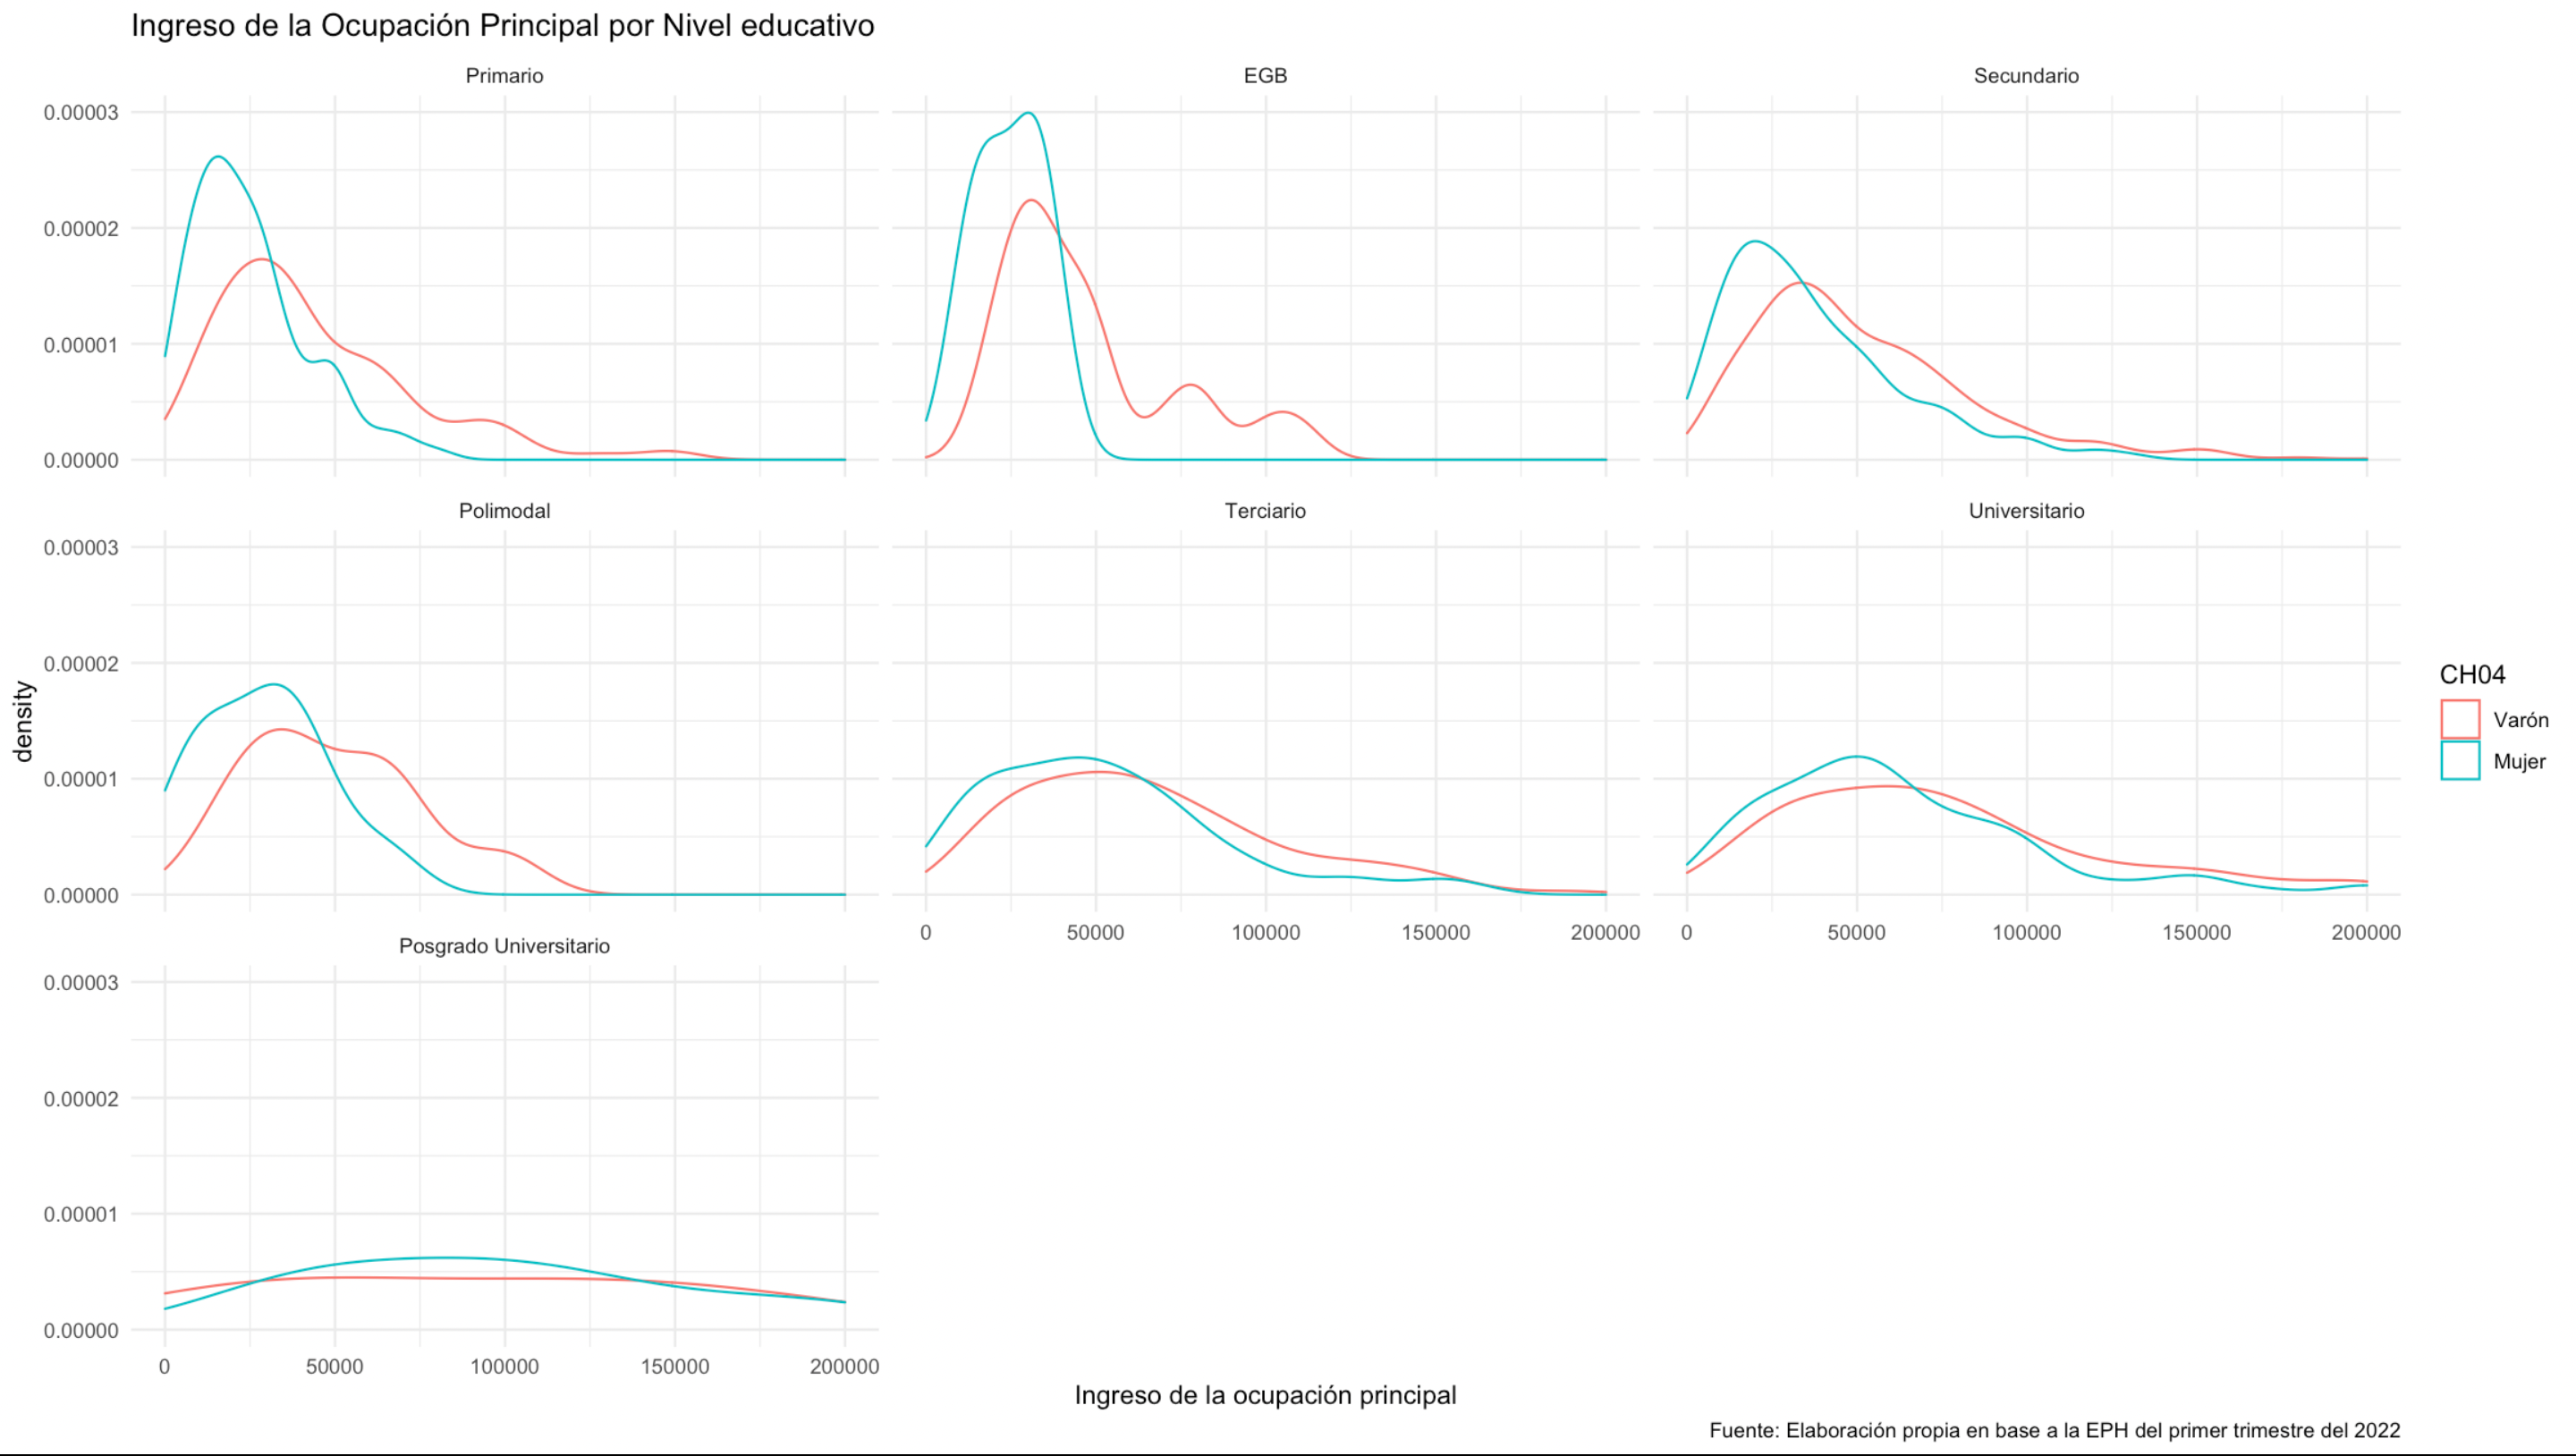
\includegraphics[scale=0.28]{figuras/kernel_por_ch12_genero.png}
    \caption{Distribución de ingreso por CH12 y género}
    \label{fig:kernel_ingreso_genero_nivel_ed}
\end{figure}


La Tabla 2 representa los salarios promedios (diferenciando aquellos que terminaron el nivel o no), la frecuencia (el porcentaje del total de las personas de ese género que alcanzaron ese nivel educativo) y la tasa de finalización (el porcentaje del total de personas de ese género que finalizaron ese nivel educativo con respecto al total de los que llegaron a ese nivel). 
\begin{table}[h]
\label{tab:my table} 
\centering
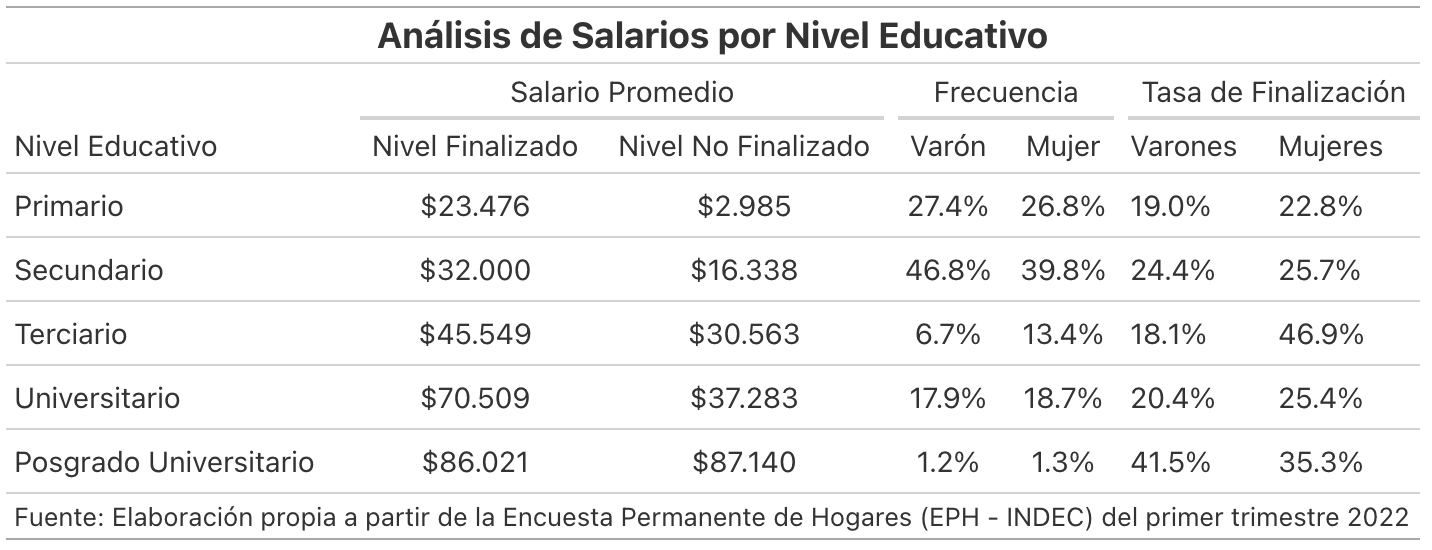
\includegraphics[scale=0.55]{figuras/tasa_finalizacion.png}
\caption{Análisis de Salarios por Nivel Educativo} 
\end{table}

La primera conclusión relevante es que terminar el nivel educativo siempre genera un incremento del ingreso con respecto a no terminarlo. Esto puede explicarse a partir del modelo de señales expuesto en el marco teórico: terminar el nivel da la señal de que se trata de un trabajador más productivo. 

En cuanto a las columnas de frecuencia y tasa de finalización, se puede extraer la conclusión de que las mujeres tienden a educarse más que los hombres ya que las mujeres con más frecuencia cursan el terciario y nivel universitario y su tasa de finalización es más alta. De todas formas, para el posgrado universitario la diferencia de frecuencia es prácticamente la misma, aunque la tasa de finalización para hombres vuelve a ser un tanto más alta. 


Cabe aclarar que no representa una diferencia significativa en la muestra terminar el posgrado universitario. Esto puede deberse a que el simple hecho de haber comenzado un posgrado es señal suficiente como para recibir el sueldo más alto. 

Respecto a la discusión de brecha salarial por nivel educativo, se construyó la Tabla 3 para entender la dinámica entre salario promedio y horas trabajadas por género. Una de las principales conjeturas que se presentan es que las mujeres ganan menos dinero en promedio, pero también trabajan menos cantidad de horas. 

\begin{table}[h]
\label{tab:my table} 
\centering
    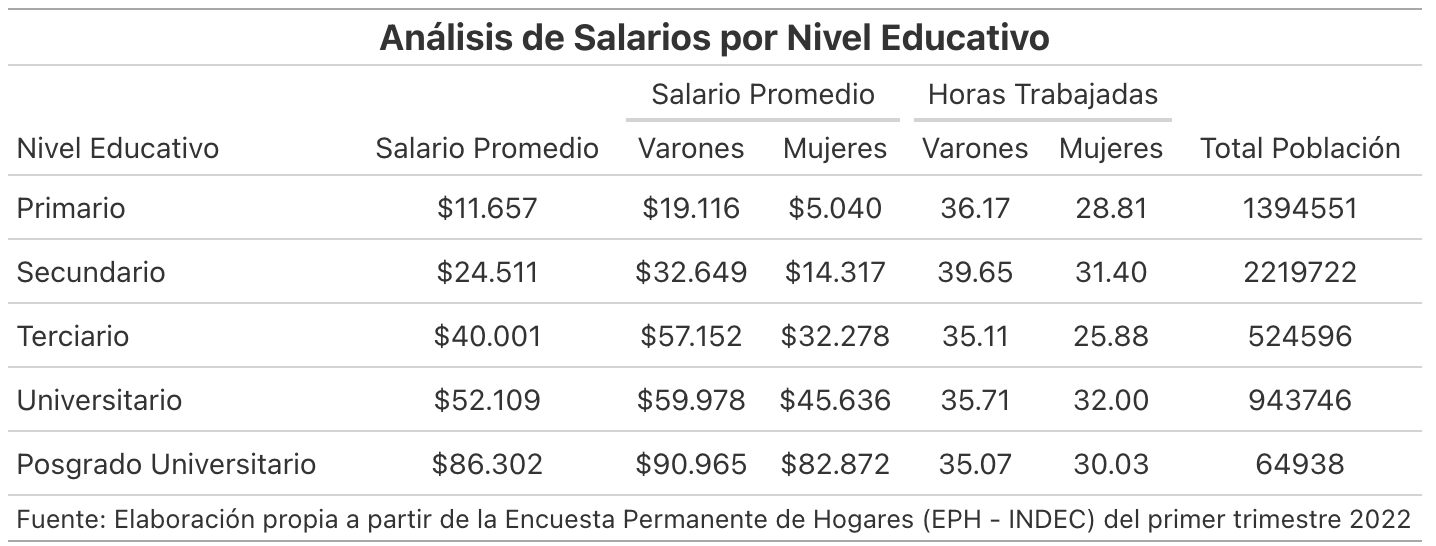
\includegraphics[scale=0.55]{figuras/analisis-salarios_mil.png}
    \caption{Análisis de Salarios por Nivel Educativo} 
\end{table}

Empíricamente, es indiscutible que a mayor nivel educativo alcanzado, en promedio, mayor es el ingreso. Sin embargo, no se está considerando el costo marginal que existe en dedicar un año adicional a educarse. Como se indicó en el Marco teórico, no solamente se trata de los costos directos como la matrícula o cuotas, sino el costo de oportunidad que se vuelve cada vez mayor. Por lo tanto, la próxima sección tendrá por objetivo calcular el retorno marginal de cada año adicional invertido en educación. 

Por lo tanto, para encarar la próxima sección, es fundamental tener presente el siguiente gráfico. 

\begin{figure}[h]
    \centering
    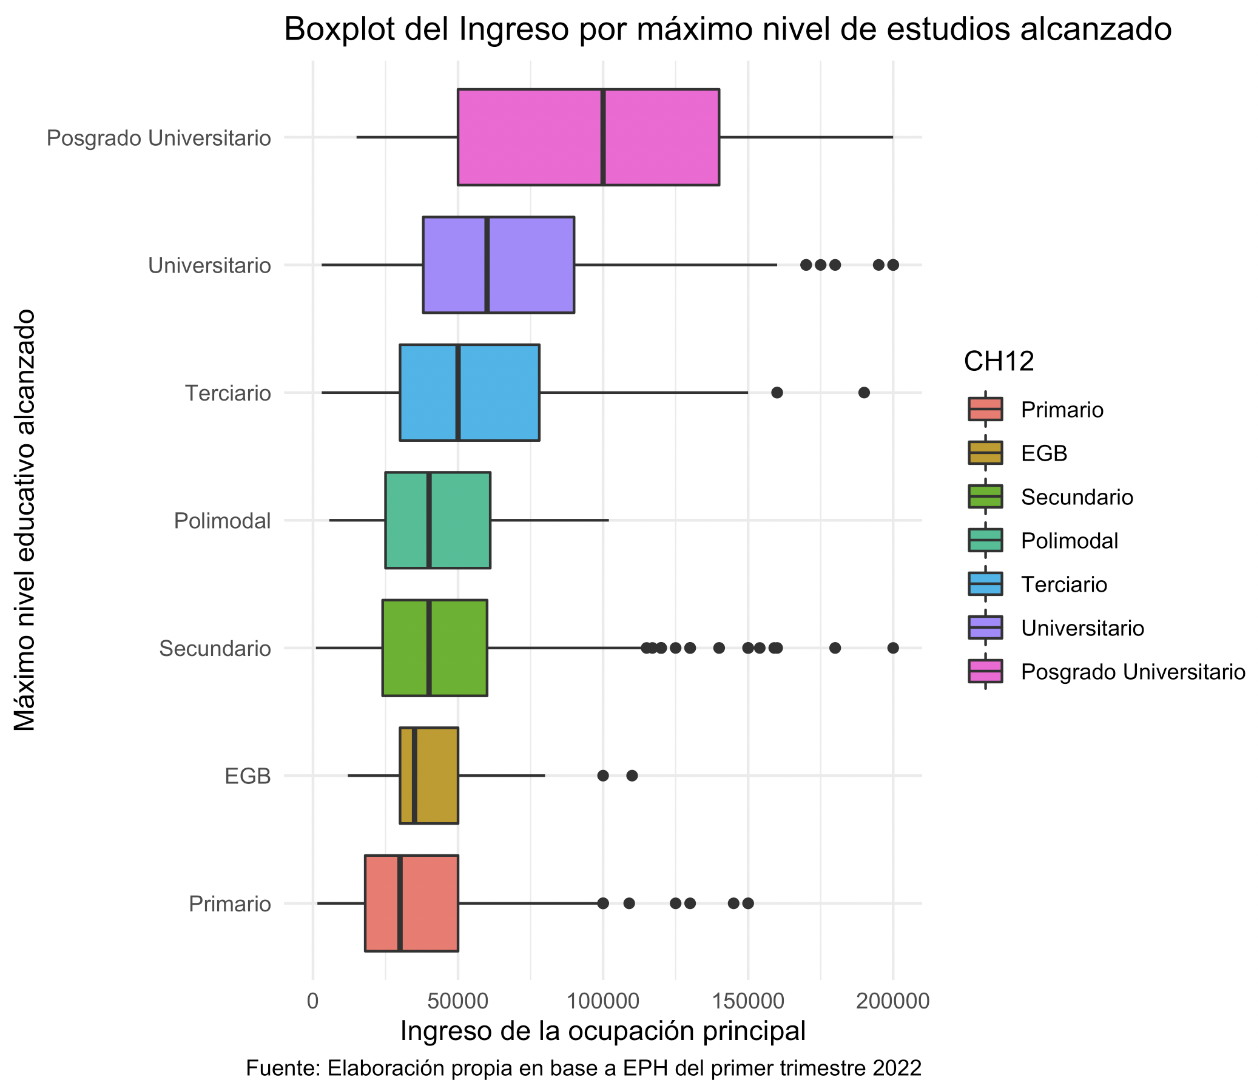
\includegraphics[scale=0.4]{figuras/CH12_boxplot.png}
    \caption{Ingreso por máximo nivel de estudio alcanzado}
    \label{fig:kernel_ingreso_genero_nivel_ed}
\end{figure}


\newpage
\section{Retornos a la Educación}
\label{sec:concepts}

\subsection{El Modelo\footnote{Este modelo está basado en Fiszbein, Giovagnoli y Patrinos (2007)}}

Siguiendo a Mincer(1974), el logaritmo natural de los ingresos es función de la educación y de la experiencia en el mercado laboral: 

\begin{equation}
    LnW_i=\alpha+\beta_1S_i+\beta_2X_i+ \beta_3X^2_i+\mu_i
\end{equation}

donde $LnW$ es el logaritmo natural del salario por hora para el i-ésimo individuo; $S_i$ son los años de educación; $X_i$ es la experiencia en el mercado laboral que es calculada como edad - años de educación promedio - 6; $X_2$ es la experiencia al cuadrado y $\mu$ refleja las habilidades no observadas.

De esta manera, $\beta_1$ puede interpretarse como el promedio de retornos a la educación (Chiswick, 1998). 

También puede estimarse retornos a la educación por nivel educativo alcanzado. Esto se puede lograr utilizando variables binarias que representan el nivel educativo.  

\begin{equation}
    LnW_i=\alpha+\beta_1 {edupc}_i+ \beta_2 {edusi}_i+\beta_3 {edusc}+\beta_4 {eduui}_i+\beta_5 {eduuc}_i+ \beta_6 X_i+\beta_7 X^2_i+\mu_i
\end{equation}

donde edupc, edusi, edusc, eduui, eduuc refieren a variables dummy para primaria completa, secundaria incompleta y secundaria completa, universitario uncompleto y universitario completo respectivamente. No está incuyendo educación primaria incompleta dado que es el regresor. 

Entonces, \textit{edupi} toma valor de 1 si no se completó la escuela primaria o no tuvo instrucción (6 años o menos); \textit{edupc} toma valor de 1 si se completó la escuela primaria (7 años de educación); \textit{edusi} toma valor de 1 si no completó la escuela secundaria (entre 8 y 11 años de educación); \textit{edusc} toma valor de 1 si el individuo completó la escuela secundaria (12 años de educación); \textit{eduui} toma valor de 1 si no se completó la educación universitaria (entre 13 y 16 años de educación); \textit{eduuc} toma valor de 1 si el individuo terminó la universidad (17 años o más).

Los retornos a la educación, por lo tanto, se derivan de la siguiente manera: 
\begin{gather*}
    r_{edupc}= \frac{\beta_1}{S_{edupc}}\\
    r_{edusi}= \frac{(\beta_2-\beta_1)}{(S_{edusi}-S_{edupc})}\\
    r_{edusc}= \frac{(\beta_3-\beta_1)}{(S_{edusc}-S_{edupc})}\\
    r_{eduui}= \frac{(\beta_4-\beta_3)}{(S_{eduui}-S_{edusc})}\\
    r_{eduuc}= \frac{(\beta_5-\beta_2)}{(S_{eduuc}-S_{edusc})}\\
\end{gather*}

donde $S_{edupc}$, $S_{edusi}$, $S_{edusc}$, $S_{eduui}$ y $S_{eduuc}$ son el total de años de escolaridad para cada nivel de educación.

Cabe destacar que este modelo toma dos supuestos importantes: (1) el diferencial de salarios entre trabajadores con distintos niveles de educación es constante a lo largo de todo el período; y (2) el único costo de continuar estudiando son los salarios no obtenidos durante ese período. Los modelos serán estimados usando MCO. 

\subsection{Los Datos}
\label{sec:concepts:sec2}

Para realizar el trabajo empírico se utilizó la Encuesta Permanente de Hogares del primer trimestre del 2022. Específicamente, para calcular los retornos a la educación nos concentraremos en las variables: NIVEL\_ED (máximo nivel educativo alcanzado), P21 (ingreso de la ocupación principal), PP3E\_TOT (horas de trabajo semanales) y CH06 (edad). Además, se filtraron los datos por ingreso laboral mayores a cero y edad entre 18 y 65 años.  

A los efectos de estimar los retornos, fue necesario construir algunas variables: $LnW_i$ es el logaritmo natural del salario mensual (P21) sobre la cantidad de horas trabajadas en el mes.  La Experiencia se construye a partir de la diferencia entre la edad, los años de escolarización y seis (la edad a la que comienza la educación formal). Como indica la Ecuación de Mincer, también se considerará los retornos a la experiencia al cuadrado. 
Los retornos a cada nivel educativo serán trabajados como fue indiciado en el apartado anterior.


\section{Resultados}
\label{sec:concepts:sec3}

En esta sección se presentarán los resultados de las regresiones de Mincer. El Modelo 1 de la Tabla 4 muestra los resultados de la Regresión (1) y el Modelo 2 los resultados de la Regresión (2) que diferencia por nivel educativo. 

La primera conclusión relevante es que \textbf{cada año de educación adicional lleva a un incremento del salario, en promedio, de 8\%}. Este número debemos compararlo con los resultados de la Tabla 1. De esta manera, tomando los retornos a la educación del 2014 para la región latinoamericana de 9.3\% (Montenegro y Patrinos, 2014), Argentina se encontraría debajo de su países limítrofes por más de un punto. 

Si se considera la literatura de los retornos a la educación argentina específicamente mencionada en la segunda sección, los retornos a la educación para inicios del siglo se encontraban en el 11\% (Fiszbein, Giovagnoli y Patrinos, 2007). La caída, entonces, de los retornos a la educación en la última década ha sido pronunciada. En contraste, el \textit{educational attainment} de la Argentina es uno de los más altos de la región (Barro y Lee, 2022) y el acceso desde el jardín de infantes hasta la universidad es público. 

Por otra parte, \textbf{cada año adicional de experiencia en el mercado laboral aumenta en un 3\% el salario}. Este número coincide con el de la literatura que aborda el tema de retornos a la educación en Argentina (Fiszbein, Giovagnoli y Patrinos, 2007). A su vez, este indica que uno esperaría que la experiencia al cuadrado sea un número pequeño y negativo, algo que también se da en el modelo estimado. 

\newpage
\begin{table}[!h]
    \centering
    \includegraphics[scale=0.75]{Mincer equation long.png}
    \caption{Resultados ecuación de Mincer y la ecuación de Mincer desagregada por nivel educativo} 
\end{table}

Para complementar este análisis, se puede estimar la Ecuación 1 de manera anual desde 2004 hasta 2022 y capturar el coeficiente 'yearse' que representa la tasa de retorno promedio al año adicional de educación. De esta manera, se obtiene la Figura 8. Resulta evidente la caída pronunciada en la tasa de retorno con picos de 11\% en 2005 y 7.5\% para 2013. 


\newpage
\begin{figure}[h]
    \centering
    \includegraphics[scale=0.4]{figuras/tasa de retornos a la educacion.png}
    \caption{Tasas de retornos a la educación a través del tiempo}
    \label{fig:my_label}
\end{figure}

En contraste, tomando la base de datos de \textit{educational attainment} de Barro \& Lee (1960-2020), la tendencia de años promedio de escolarización es creciente. 

\begin{figure}[h]
    \centering
    \includegraphics[scale=0.4]{figuras/años de escolarizacion promedio tendencia.png}
    \caption{Años de escolarización promedio a través del tiempo}
    \label{fig:my_label}
\end{figure}

En definitiva, se encuentra una aparente contradicción en tanto los retornos a la educación son más bajos, pero en promedio se educan más años. 



\newpage
\section{Conclusión}

Luego de haber calculado los retornos a la educación siguiendo la Ecuación de Mincer para Argentina en el primer trimestre de 2022 y anualmente para el período 2004-2021, se puede concluir que la inversión en capital humano incrementa los ingresos laborales de los individuos de manera estadísticamente significativa. La estimación arrojó un resultado de una tasa de retorno del 8\% para el 2022 y un retorno a la experiencia de 3\% por año. Introduciendo al análisis los años de escolarización promedio y comparando con la serie de retornos, se desprende una observación paradójica: la tendencia de los retornos a la educación es decreciente mientras que los años de escolarización están en aumento.  

Por un lado, esto puede estar relacionado con el contexto histórico. La reforma educativa de la década de 1990 \footnote{Ley Nº 24.195 (La Ley Federal de Educación, 1993) y Ley Nº 24.521 (Ley de Educación Superior, 1995).} representó un cambio en la orientación de las políticas públicas educativas y tenía por objetivo una mejora institucional del sistema. No obstante, terminó haciendo más accesible el pasaje de año y generando las condiciones para un declive paulatino en el sistema educativo en general (Tedesco y Fanfani, 2001). Por lo tanto, una explicación plausible es que, como en promedio se educan más años, marginalmente valga menos el año de educación adicional. Además, si la educación de relativamente menor calidad, la señal también es peor, y sería necesario acceder a un nivel superior para dar la misma señal de productividad. 

Por otro lado, como se mencionó en la sección 3, los salarios son nominalmente muy bajos en la Argentina (el ingreso laboral promedio ronda los \$300 dólares)  y genera incentivos muy fuertes a lo que se conoce como la 'fuga de cerebros'. Este término alude a la pérdida de capital humano de un área a otra o de una industria a la otra. Normalmente tiene lugar cuando individuos calificados y profesionales dejan su país natal para ir a algún otro donde puedan sacar provecho de las mejores oportunidades.

Esta pérdida de trabajadores calificados puede darse de distintas maneras, pero principalmente como emigración. Dada las estadísticas de la Dirección Nacional de Migraciones, los principales destinos de emigración para los argentinos tienden a ser España, Italia y Estados Unidos. Asimismo, con el fortalecimiento del trabajo remoto en los últimos años, es una alternativa muy buscada trabajar para otro país viviendo desde Argentina. La EPH no puede capturar a los individuos educados que emigraron, pero sí podría explicar una parte de la caída de los retornos. 

Un punto de suma relevancia que excede a este trabajo, pero es relevante para un análisis futuro, es si esta reducción de la tasa de retornos a la educación es causa o consecuencia de la pérdida de capital humano. Se trata de que los individuos más capacitados ven en el exterior más retorno a su inversión y deciden irse del país o, como se van del país, el retorno a la educación es menor. 

En definitiva, cualquiera sea la causa de la caída a los retornos a la educación, la situación es crítica. Con una escasez inminente de mano de obra calificada, la solución educativa es necesaria, aunque rara vez considerada por los gobiernos de turno, y deberá estar acompañada por políticas macroeconómicas acordes que disminuyan los incentivos a que los individuos más educados a dejen el país.  

\newpage
\section{Anexos}
\subsection{Anexo 1: el mercado laboral argentino}

Antes de comenzar a analizar la distribución del ingreso en particular, es relevante explicar el mercado laboral argentino en general. En el Anexo 1 se desarrolla un análisis más exhaustivo de los principales indicadores laborales en Argentina, pero a continuación se presentan las principales conclusiones en Figure \ref{fig:distribucion_del_ingreso}. 

\begin{figure}[h]
    \centering
    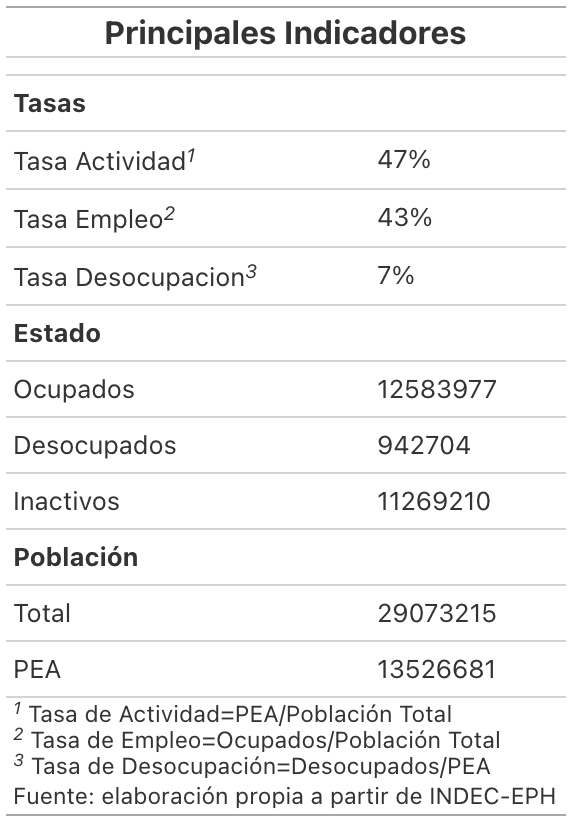
\includegraphics[scale=0.7]{figuras/principales_indicadores_mercado_laboral_2022.png}
    \caption{Principales indicadores del mercado laboral para el primer trimestre de 2022}
    \label{fig:distribucion_del_ingreso}
\end{figure}
\begin{itemize}
        \item \textbf{Condición de actividad: }relación de las personas con la producción de bienes y servicios con valor económico en el mercado.
\begin{itemize}
        \item \textbf{Ocupado}: quienes se encuentran trabajando en la semana de referencia o no trabajando pero manteniendo un puesto de trabajo.
        \item \textbf{Desocupado}: quienes no tienen trabajo, están disponibles para trabajar y buscan trabajo activamente en algún momento de los últimos 30 días.
        \item \textbf{Inactivo}: quienes no se encuentran trabajando ni buscaron activamente trabajo en el período de referencia -últimos 30 días-.
 \end{itemize}
 \end{itemize}
 \begin{itemize}
 \item  \textbf{Tasa de actividad:} calculada como porcentaje entre la población económicamente activa y la población total de referencia.
\item  \textbf{Tasa de empleo:} calculada como porcentaje entre la población ocupada y la población total de referencia.
\item \textbf{Tasa de desocupación:} calculada como porcentaje entre la población desocupada y la población económicamente activa.
\item \textbf{Tasa de ocupados demandantes de empleo:} calculada como porcentaje entre la población de ocupados demandantes de empleo y la población económicamente activa.
 \end{itemize}


\subsection{Anexo 2: la informalidad en el mercado laboral argentino}

La Encuesta Permanente de Hogares tiene como uno de sus principales propósitos, ser un indicador de la tasa de informalidad. Más allá de que los encuestados no declaran explícitamente que sean formales, algunas de las preguntas hacen referencia a si tienen descuento jubilatorio(PP07H), vacaciones pagas(PP07G1),  aguinaldo(PP07G2), días pagos por enfermedad(PP07G3) y obra social(PP07G4). Estas son condiciones que hacen que un trabajador sea formal dada la Ley 20.744 y las variables indicadas entre paréntesis son las que se refieren a las respuestas de esas preguntas en la base de microdatos. 

Países desarrollados tienen menos de 20\% de tasa de informalidad, pero en Argentina ronda el 40\%. Una de las conclusiones evidentes que puede desprenderse de este trabajo es que a mayor educación, menor nivel de informalidad. 

A partir de los datos del primer trimestre de cada año, se puede demostrar que esto es cierto:

\begin{figure}[h]
    \centering
    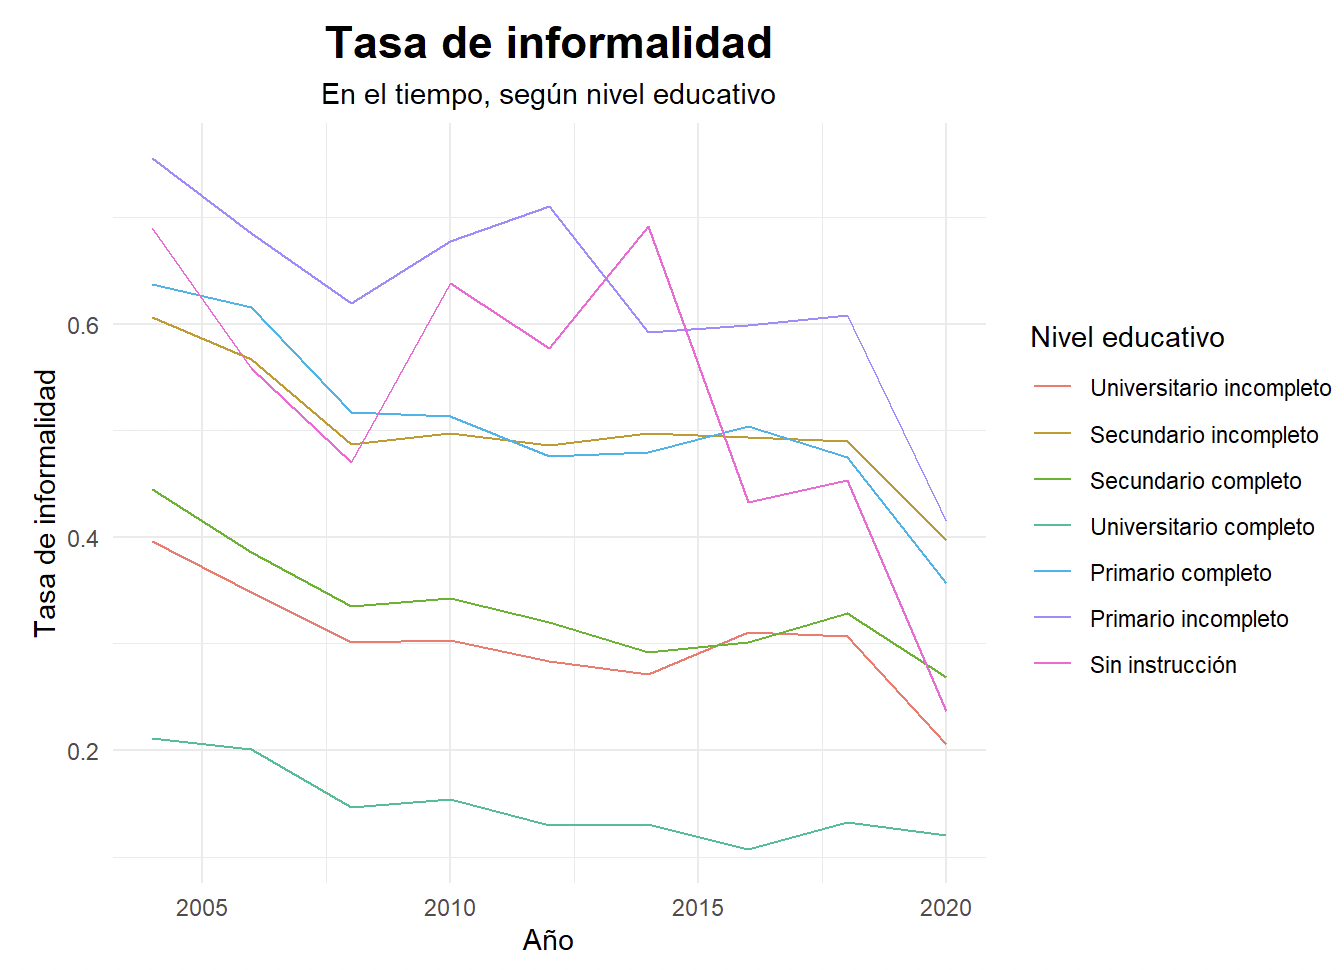
\includegraphics[scale=0.5]{figuras/tasa de informalidad por nivel educativo.png}
    \caption{Tasa de Informalidad por Nivel Educativo}
    \label{fig:my_label}
\end{figure}

\newpage
\section{Referencias}
\begin{itemize}
    \item Adrogué, C. (2006). Desempleo y retornos a la educación superior en la Argentina (1974-2002). \textit{Universidad Católica de Salta, Salta: XLI Reunión Anual de la Asociación Argentina de Economía Política.}
    
    \item Arrow, K. J. (1973). \underline{Information and economic behavior}. Harvard University Press.

    \item Barro, R. J., \& Lee, J. W. (1996). International measures of schooling years and schooling quality. \textit{The American Economic Review}, 86(2), 218-223.

    \item Becker, G. S. (1964). \underline{Human capital theory}. Columbia, New York,1964.

    \item Borjas, G. J., \& Van Ours, J. C. (2020).\underline{Labor economics}. Boston: McGraw-Hill/Irwin.

    \item Card, D. (1994). \textit{Earnings, schooling, and ability revisited}. NBER Working Papers Series, N° 4832.

    \item Coremberg, A. (2010). The Economic Value of Human Capital and Education in an Unstable Economy: Argentina. \textit{In 31st General Conference of The International Association for Research in Income and Wealth.}
    
    \item Fiszbein, A., Giovagnoli, P. I., \& Patrinos, H. A. (2007). Estimating the returns to education in Argentina using quantile regression analysis: 1992-2002.\textit{Económica}, 53.
    
    \item Griliches, Z. (1977). Estimating the returns to schooling: Some econometric problems. \textit{Econometrica: Journal of the Econometric Society}, 1-22.

    \item Mincer, J. (1974). Schooling, Experience, and Earnings. Human Behavior \& Social Institutions No. 2. NBER, New York.

    \item Montenegro, C. E., \& Patrinos, H. A. (2014). Comparable estimates of returns to schooling around the world. World Bank policy research working paper, (7020).

    \item Paz, J. A. (2009). Retornos a la educación en Argentina. Estructura regional.\textit{Documentos de trabajo del IELDE}, 1-39.

    \item Psacharopoulos, G., \& Patrinos, H. A. (2018). Returns to investment in education: a decennial review of the global literature.\textit{Education Economics}, 26(5), 445-458.

    \item Schultz, T.W. (1961). “Investment in Human Capital”, \textit{American Economic Review LI: 1-17}.

    \item Spence, M. (1973) “Job Market Signaling” \textit{The Quarterly Journal of Economics}, 87 (3): 355-374.
    
    \item Tedesco, J. C., \& Tenti Fanfani, E. (2001). La reforma educativa en la Argentina. Semejanzas y particularidades. \textit{Buenos Aires: Ministerios de Educación de Argentina, Chile y Uruguay, Grupo Asesor de la Universidad de Stanford/BID}.

    \item Todaro, M. P., \& Smith, S. C. (2020). \underline{Economic development}. Pearson UK.

\end{itemize}


\end{document}